\documentclass[11pt]{article}

\setlength{\textwidth}{6.0in}
\setlength{\oddsidemargin}{23pt}
\setlength{\evensidemargin}{23pt}
\setlength{\topmargin}{-0.5in}
\setlength{\textheight}{8.5in}
\renewcommand{\thefigure}{\arabic{figure}}

\usepackage[dvips]{graphicx}
\DeclareGraphicsExtensions{.ps,.jpg,.eps,.ps,.pdf}

\usepackage{fancybox} % For making Oval borders.
\usepackage{amssymb}  % For, for example, \mathbb, \big, and \mapsto
\usepackage{url} % For email addresses, hypertext links, ...
\usepackage{color} % For color.
\usepackage{hyperref} % For hyper reference but *essential* for seminar.

% Options for hyperref.

\hypersetup{pdfpagemode=none,pdfstartview=FitH} % For the initial view.
\hypersetup{colorlinks=true}
\hypersetup{hypertexnames=false} % Eliminates message: pdfTeX warning (ext4)
\hypersetup{urlcolor=red}

% Abbreviations

\newcommand{\tron} {\mbox{\sf \footnotesize TRON}}
\newcommand{\icfs} {\mbox{\sf \footnotesize ICFS}}
\newcommand{\tao} {\mbox{\sf \footnotesize TAO}}
\newcommand{\cops} {\mbox{\sf \footnotesize COPS}}
\newcommand{\gpcg} {\mbox{\sf \footnotesize GPCG}}

\begin{document}

\setlength{\baselineskip}{15pt}

\begin{center}
{\large
\textbf{Toolkit for Advanced Optimization}}
\end{center}

\href{http://www.mcs.anl.gov/tao}
{The Toolkit for Advanced Optimization} (\tao)
focuses on the design and implementation of
component-based optimization software for the
solution of large-scale optimization applications
on high-performance architectures.
Our approach is motivated by the
scattered support for parallel computations and
lack of reuse of linear algebra software in
currently available optimization software.
Our design enables connection to lower-level
support (parallel sparse matrix data
structures, preconditioners, solvers) provided in toolkits such as
\href{http://www.mcs.anl.gov/petsc}{PETSc},
and thus we are able to build on top of these toolkits
instead of having to redevelop code. The advantages in
terms of development time are significant.

\begin{figure}[h]
\centerline {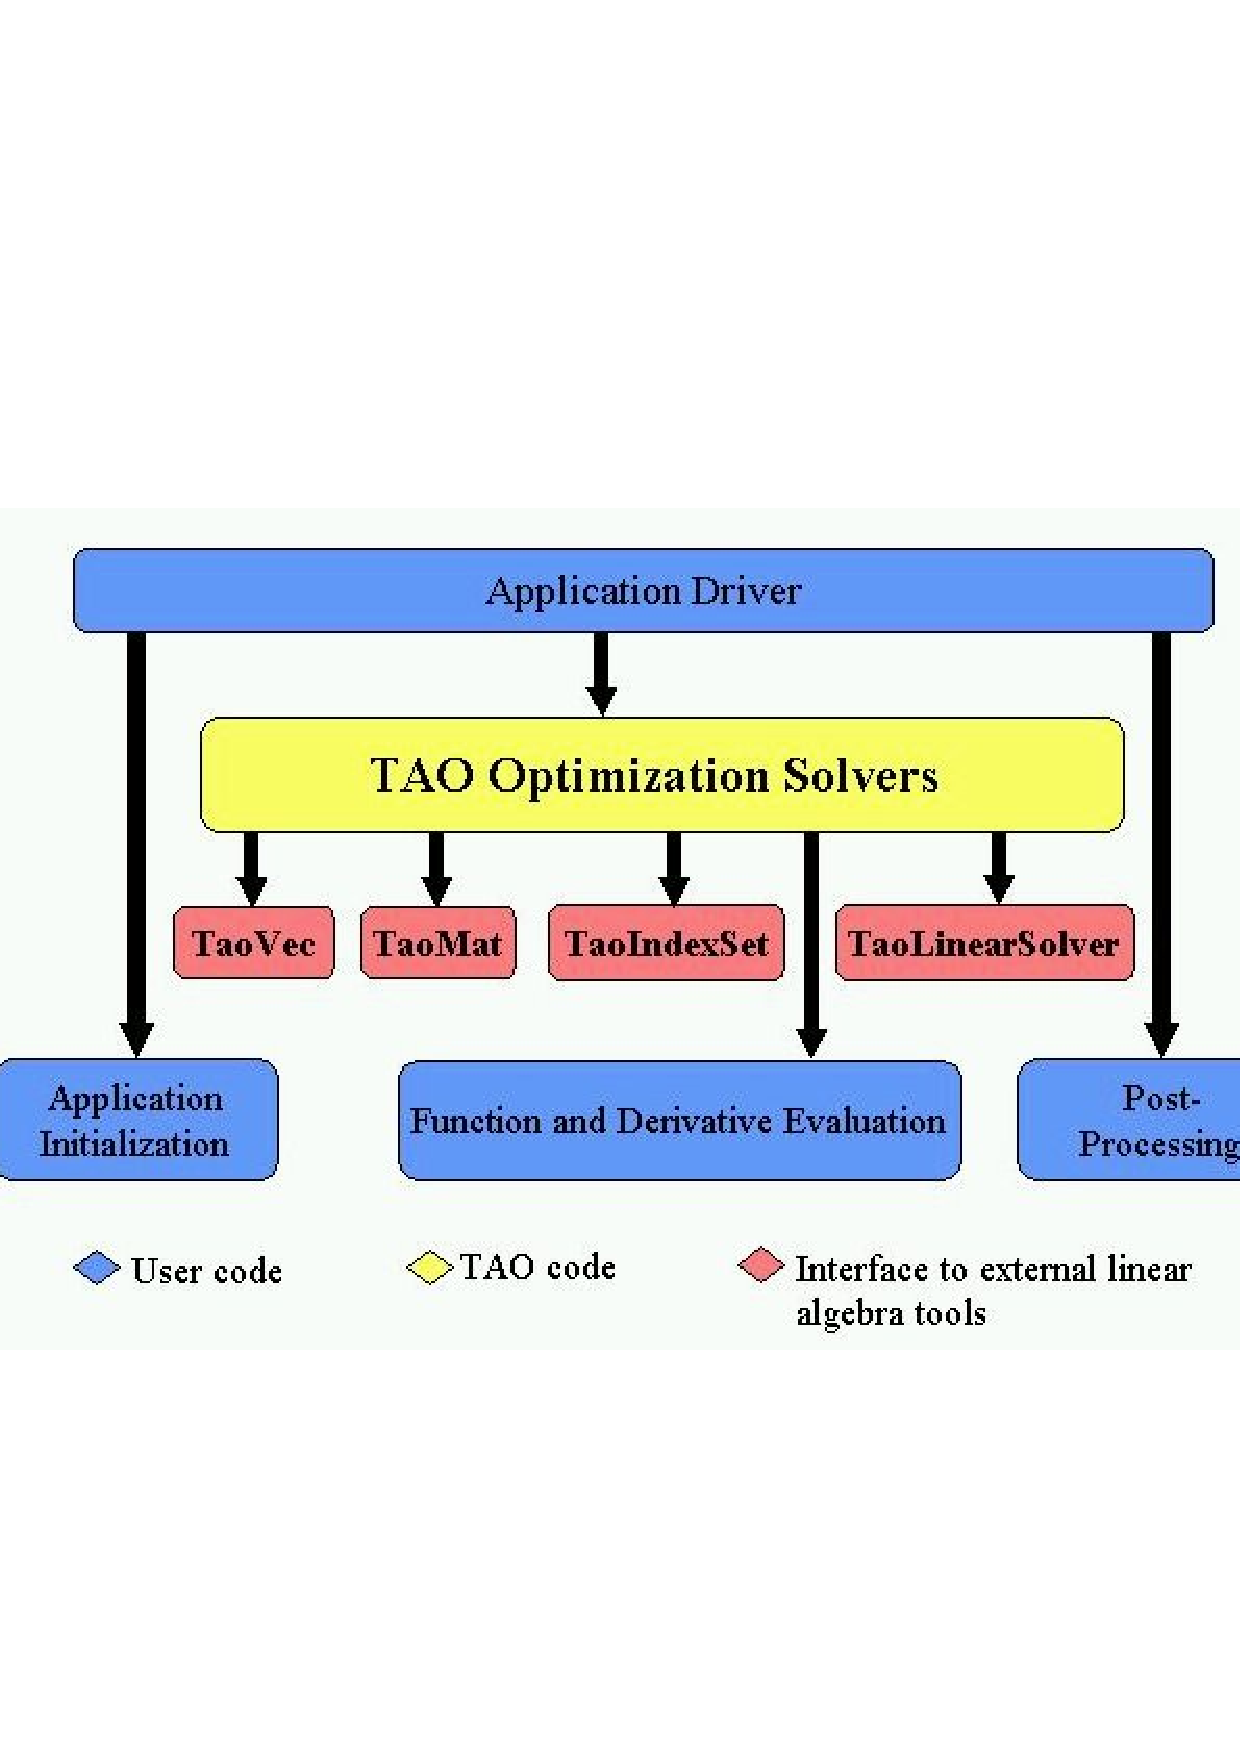
\includegraphics[width = 5.8in]{tao_comps}}
\caption{\tao\ Components}
\label{figure:tao_comps}
\end{figure}

Version 1.2 of \tao, released in June 2001, is a major accomplishment.
As can be seen by the \tao\ components in
Figure~\ref{figure:tao_comps}, we employ external tools for linear
algebra.  In particular, version 1.2 introduces new \tao\
abstractions, including \texttt{TaoVec}, \texttt{TaoMat},
\texttt{TaoIndexSet}, and \texttt{TaoLinearSolver}, instead of our
previous approach of directly using the counterparts within PETSc.
This new design enables us to interface to a variety of underlying
linear algebra toolkits, including those that support the emerging
Equation Solver Interface (ESI) standard.  As a result,
interoperability with other software components is dramatically
improved so that we may more easily leverage a broader range of
sparse linear solver technology.

At the algorithmic level, the major improvements in version 1.2 of \tao\
are  an improved limited-memory conjugate gradient algorithm
and two new solvers for mixed  complementarity problems.
On our recent benchmark tests, the 
limited-memory conjugate gradient algorithm outperforms all
other (single-processor) conjugate gradient algorithms.
The addition of mixed complementarity solvers to \tao\
introduces a new capability that is not available in other
optimization packages.

We have also continued to improve the 
\href{http://www.mcs.anl.gov/tao}{\tao\ web site}, which
includes the
complete source code and documentation, as well as benchmarks and tutorials.
The HTML version of the documentation is of special note
since the sample programs have cross-references
to function definitions.


%  \bibliographystyle{siam}

%  \bibliography{../tao,%
%  /home/more/papers/bibs/opt80,%
%  /home/more/papers/bibs/opt90,%
%  /home/more/papers/bibs/opt00}%

\end{document}

